
\todo {Things that need to be done for the plots}
\begin{itemize}
	\item (Plots) Shape comparisons of main analysis variables for CR3, CR2, SR (Gives the idea of the uncertainty)
	\item (Table) Cross section limits of 7 TeV studies (Just put al the numbers in the formula)
\end{itemize}

\begin{itemize}
	\item Brief introduction of the chapter content
	\item State that everything is based on the 7 TeV studies and will go in details on the differences
\end{itemize}



\section{Signal and background samples}

\begin{itemize}
	\item List of samples used for the studies
	\item brief details on how the signal samples has been generated and how data is stored now (miniaods), everything on the production chain (if too much refers to appendix)
\end{itemize}



\section{Object reconstruction}
\begin{itemize}
	\item make clear the experiment will gain access to a trigger triggering only on di-jet properties (no MET Lvl 1 seed like for 7 TeV)
	\item Dijet delta eta cut removed (obsolete because strongly correlated to the $m_{jj}$ cut) 
	\item $m_{jj}$ cut removed (chosen variable for cuts optimization), be aware of the fact that there's gonna be an online cut coming from the chosen trigger anyway.
	\item \hadtau isolation requirement has still high impact on statistics
	\item mention new b-jet and lepton veto used (reference to internal notes if necessary)
\end{itemize}

During the technical stop the experiment underwent through several updates on both hardware and software side. This	translates also into an updated version of the physical object definition used for this study with respect to the one used in the 7\tev analysis.

The \hadtau object reconstruction went through a major update with the introduction of new isolation and decay mode discriminators and electron veto \cite{bib:TauID_13tev}. The new \hadtau object reconstruction has been commissioned for $\pt > 20$\gev ad in all $\eta$ ranges. By using the specifications suggested by the Tay POG there's an increase of the overall TauID efficiency of about 10\% for loose isolated \hadtau with respect to the 7\tev specifications, going up to 71\% for $Z \longrightarrow\tau\tau$ events\cite{bib:TauID_13tev}. A detailed list of the \hadtau object selection can be found on Table \ref{table:tauobjdefinition_13TeV}. 

The Jet object definition remained unchanged.  

With Run 2 the experiment will gain access to a new trigger list. The aim is to use a trigger that is exclusively making an online selection on the di-jet object kinematic properties. Differently with the 7\tev trigger version this trigger can't be seeded by a level one trigger based on \met. The drop of all online selections over the \hadtau properties leads to some important advantages Firstly it is possible to have a lower \hadtau \pt selection. Secondly it is possible to go from a 1-prong to a 3-prong decay selection since this stringent requirement is not part anymore of any level 1 trigger seed. 



\section{Cross section limit studies}

The aim of this study is to optimize the event cuts is order to exclude signal at the lowest cross section measurable. A cross section limit is made my setting the significance $\alpha$ to:

\begin{equation}
\alpha = 2
\label{eq::significance_xsec_limit}
\end{equation}

There are several however definitions of significance $alpha$ available in literature. The one picked for this 13\tev study is a frequentist definition based on completely standard concepts\cite{Punzi:2003bu} is generally applicable, and has a very clear interpretation. It is particularly suitable for optimization, being independent of a-priori expectations about the presence of a signal, thus allowing the determination of a single set of cuts that is optimal both for setting limits and for making a discovery. The definition of sensitivity is:

\begin{equation}
\alpha = \dfrac{S}{\dfrac{a}{2} + \sqrt{B + (0.5 \cdot B)^{2}}}
\label{eq::punzi_formula}
\end{equation}

with $a$ as the confidence level expressed in terms of $\sigma$, $S$ and $B$ are respectively the number of signal and background vents for a given selection. One of the most important features of \autoref{eq::punzi_formula} is non-diverging in case of $B = 0$.

The number of signal events can be defined as:

\begin{equation}
S = \epsilon \cdot \sigma_{sec} \cdot L
\label{eq::punzi_signal_events}
\end{equation}

with $\epsilon$ as the efficiency for a given selection criteria, $\sigma_{sec}$ as the cross section of the signal process considered and $L$ and the luminosity given by the experiment. Is it possible now to define the efficiency $\epsilon$ as function of variables used in the analysis event selection. Three of the most important variables in the 8\tev analysis has been chosen as variables for the study: $Pt_{\tau}$,\met and $m_{jj}$. The definition of $\epsilon$ given in \autoref{eq::punzi_signal_events} now becomes:

\begin{equation}
\epsilon ( Pt_{\tau} , m_{jj} ,  \met ) = \dfrac{N_{passed}(Pt_{\tau} , m_{jj} ,  \met)}{N_{total}}
\label{eq::punzi_efficiency}
\end{equation}

with $N_{passed}$ as the number of signal events passing the selection criteria as function of the given variables and $N_{total}$



\begin{itemize}
	
	\item Background prediction in SR: two-fold ABCD method involving 2 different (Schematic rappresentation needed) correction factors
	\item LtoT conversion factor:
	\begin{itemize}
		\item Events with at least 4 jets;
		\item $NLto2T = A * B$;
		\item A: (the matched tau is also tight isolated)/(at least one jet matched to a loose tau)
		\item B: (the matched tau is also tight isolated)/(at least one jet matched to a tau (no iso requirement))
	\end{itemize}
		\item VBF conversion factor: same as before (Excluding removed cuts)
		\item Min cross section for $m_{jj} < 200$ and $130 < \met < 150$;
		\item Need to show impact of the $Pt_{\tau}$ over the limit.
		\item Uncertanties over the conversion factors (Taken from sape comparison)
\end{itemize}

\begin{figure}[tbh!]
	\centering
	\begin{tabular}{cc}
		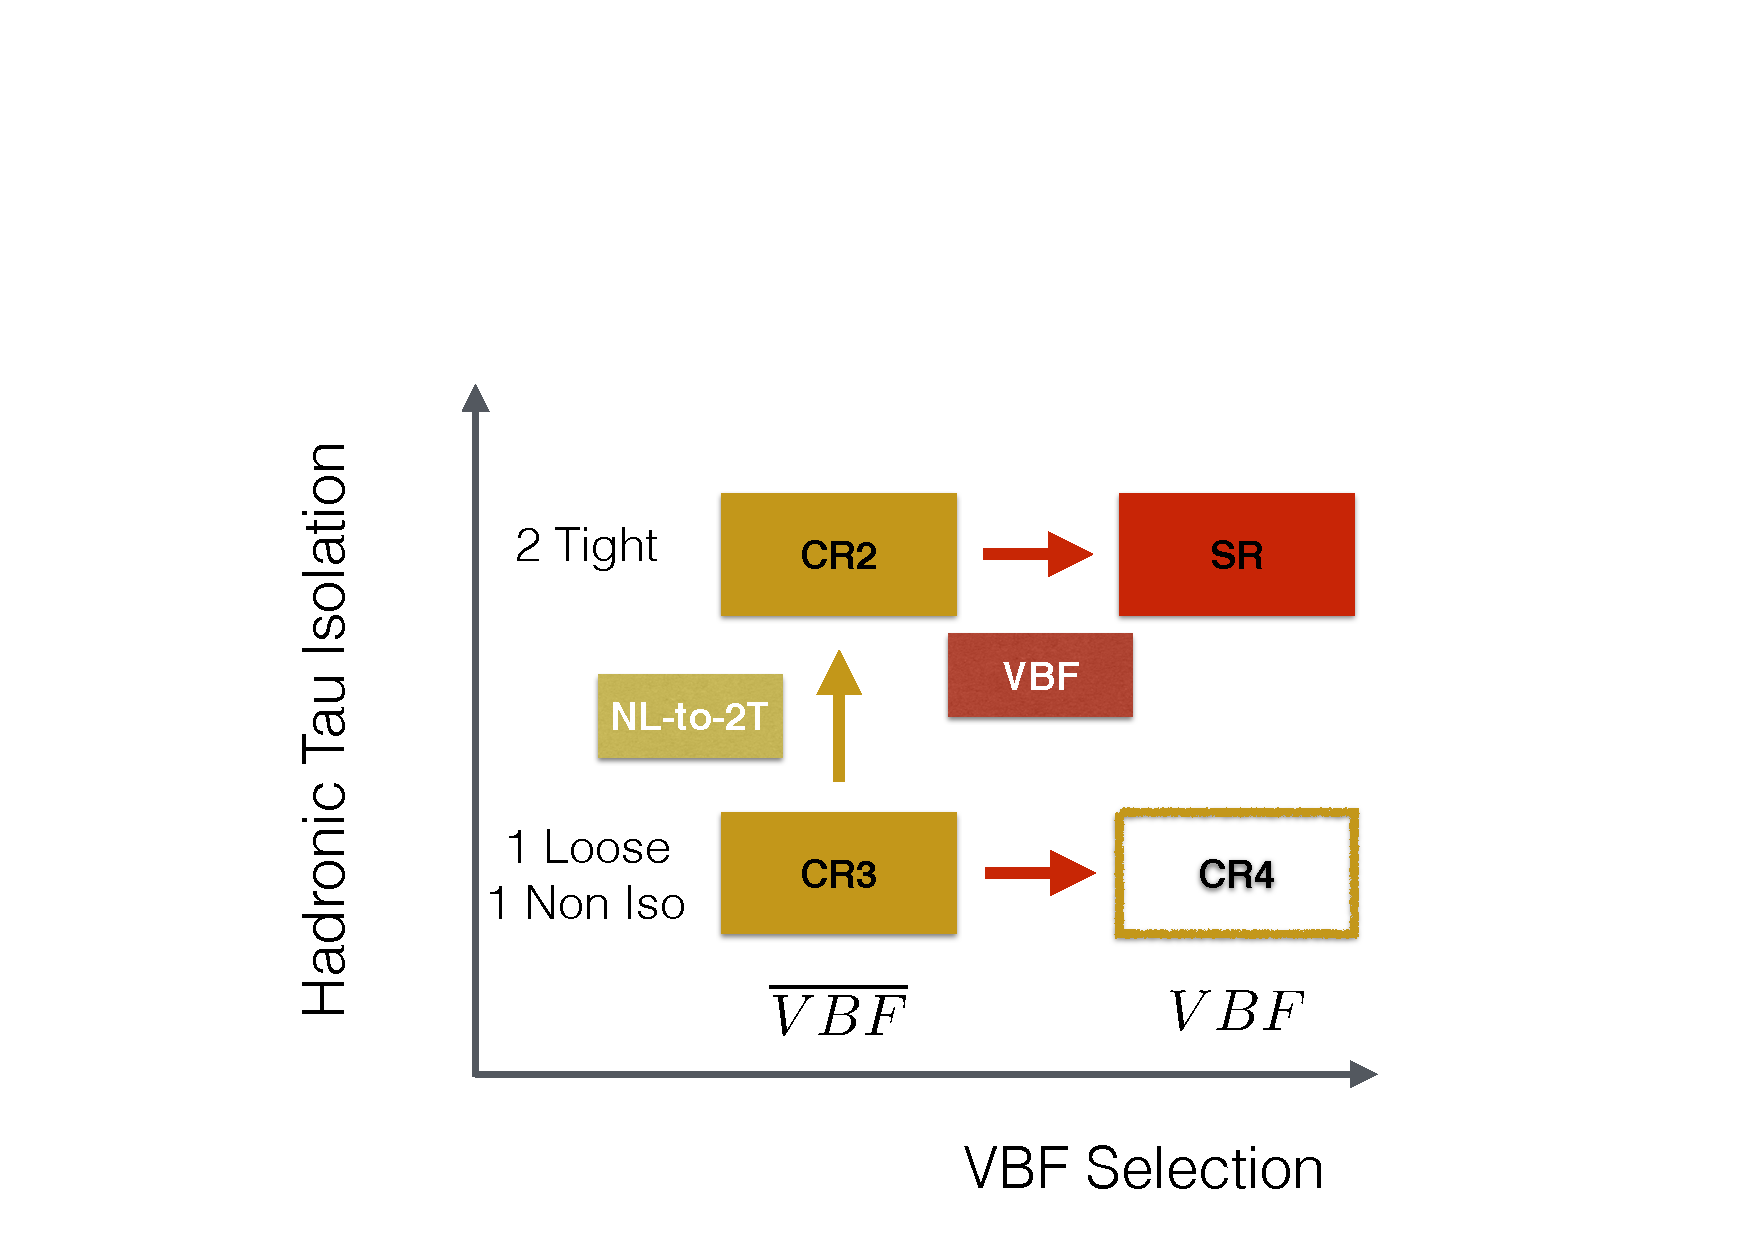
\includegraphics[width=0.75\textwidth]{PLOTS/diTauHadLSotherPlots/controlregions13TeV.pdf}
	\end{tabular}
	\caption{Definition of Signal and Control Regions using different $\hadtau$ isolation criteria and VBF selection.}
	\label{fig:crs_13tev}
\end{figure}